% !Mode:: "TeX:UTF-8"%確保文檔utf-8編碼
\documentclass{standalone}
\usepackage{tikz}
\usepackage{pgfplots}
\pgfplotsset{compat=newest}
\usetikzlibrary{decorations.pathreplacing}

\begin{document}
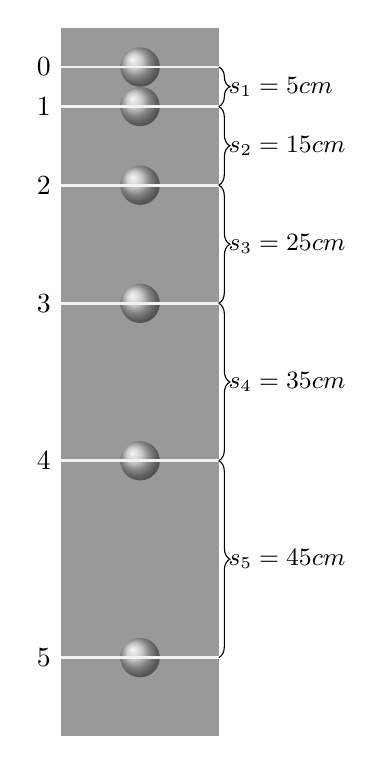
\begin{tikzpicture}

\fill[fill=black!40] (0,0) rectangle (2,-9);

\foreach \x [count=\i] in {0,0.5,1.5,3,5,7.5}{
\shade[ball color=gray!50,yshift=-\x cm] (1,-0.5) circle (0.25);
\draw[color=gray!10,line width =1pt,yshift=-\x cm] (0,-0.5) node[left,color=black] {\pgfmathprint{int(\i-1)}} -- (2,-0.5) node (\i) {};
}

\draw [decorate,decoration={brace,amplitude=4}] (1.base) to node[right] {\small $s_1=5cm$} (2.base);
\draw [decorate,decoration={brace,amplitude=4}] (2.base) to node[right] {\small $s_2=15cm$} (3.base);
\draw [decorate,decoration={brace,amplitude=4}] (3.base) to node[right] {\small $s_3=25cm$} (4.base);
\draw [decorate,decoration={brace,amplitude=4}] (4.base) to node[right] {\small $s_4=35cm$} (5.base);
\draw [decorate,decoration={brace,amplitude=4}] (5.base) to node[right] {\small $s_5=45cm$} (6.base);

\end{tikzpicture}
\end{document}